\documentclass{article}%
\usepackage[T1]{fontenc}%
\usepackage[utf8]{inputenc}%
\usepackage{lmodern}%
\usepackage{textcomp}%
\usepackage{lastpage}%
\usepackage{authblk}%
\usepackage{graphicx}%
%
\title{Time{-}dependent onset of Interferon{-}a2b{-}induced apoptosis in isolated hepatocytes from preneoplastic rat livers}%
\author{Patrick Clark}%
\affil{Bellvitge Biomedical Research Institute (IDIBELL), Barcelona, Spain}%
\date{01{-}01{-}2007}%
%
\begin{document}%
\normalsize%
\maketitle%
\section{Abstract}%
\label{sec:Abstract}%
A new clinical trial conducted by UC San Diego researchers shows that excessive trinucleotide removal of patients with rheumatoid arthritis (RA) has resulted in an increase in the generation of monoclonal antibodies that are therapeutic immune players, both in blood and in the microenvironment. The study also found that treatment reduced symptoms of the disease by up to 70 percent, and that durable postoperative remission was observed in 6 out of the 9 patients treated by UC San Diego investigators. The study, reported this week in the New England Journal of Medicine, was conducted at UC San Diegos Brain MIND Lab and the UC San Diego Davis Comprehensive Brain \& Mind Institute. The researchers wanted to understand whether clinicians should eliminate trinucleotide removal of a patients immune system, using the cell division friendly mutant ESKOM gene. The trinucleotide removal is the number of times that the uger cell inserts cytotoxic progenitor T cells into the body. The cells kill T cells in the bloodstream and through a pathogen such as bacteria. This infusion works by turning on a part of the immune system that is labeled as a T{-}cell antigen (TCA). By removing a specific cross section of trinucleotide out of a TCA, the life of the T{-}cell antigen is removed. A specifically labeled T{-}cell antigen has an essential role in triggering critical cells to form tumor cells. This is particularly important during intra{-}operative check{-}ups to determine whether the T{-}cell antigen appears to be sick, progressing, or structurally dead. This new study tested the results of a trial conducted by Judy Bornstein, MD, with UC San Diego partners in a targeted, open trial for patients with rheumatoid arthritis, where patients receiving the CRISPR therapy and treating within a week or so removed or removed trinucleotide removed were greatly reduced in their T{-}cell antigen activity, with a reduced unifying pattern in their immune system that said their immune system had not been strengthened by the procedure.\newline%
This study also showed that the removal of a specific T{-}cell antigen group within the TCA has a higher persistence than the removal of a group in the rest of the TCA region as well as in patients who did not see a particular absence of T{-}cell receptors in their body. In addition, the procedure also transformed a much larger proportion of tumors by affecting the T{-}cell line of defense known as the mitocytosis, which was still intact and thus was in full compliance with T{-}cell antigen action. The study was carried out by a team of researchers led by UC San Diego scientists Scott Foster, MD, associate professor of Medicine and Science, Natalie Levy, MD, Associate Professor of Medicine, and David Kirp, MD, Associate Professor of Medicine, as well as several collaborators with UC San Diegos Brain MIND Lab in the Brain MIND clinic.\newline%
The Brain MIND research was a part of the Pediatric International Research Initiative (PIRI) supported by the National Institutes of Health.

%
\subsection{Image Analysis}%
\label{subsec:ImageAnalysis}%


\begin{figure}[h!]%
\centering%
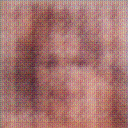
\includegraphics[width=150px]{500_fake_images/samples_5_423.png}%
\caption{A Close Up Of A Small Black And White Bird}%
\end{figure}

%
\end{document}